
\section{Final Tips \& Advanced Topics}

\begin{frame}[fragile]{Bibliography Basics}
     \begin{columns}
          \begin{column}{0.5\textwidth}
               \begin{lstlisting}
% Manual bibliography
\begin{thebibliography}{9}
     
     \bibitem{lamport94}
     Leslie Lamport,
     \emph{\LaTeX: A Document Preparation System}.
     Addison Wesley, Massachusetts,
     2nd Edition,
     1994.
     
     \bibitem{knuth84}
     Donald E. Knuth,
     \emph{The \TeX book}.
     Addison Wesley, Massachusetts,
     1984.
     
\end{thebibliography}

% In-text citation
According to Lamport~\cite{lamport94},
\LaTeX{} is...
               \end{lstlisting}
          \end{column}
          
          \begin{column}{0.5\textwidth}
               \textbf{Manual bibliography:}
               \begin{itemize}
                    \item \texttt{thebibliography} environment
                    \item \texttt{\{9\}} - width hint (number of entries)
                    \item \texttt{\textbackslash bibitem\{key\}} - define reference
                    \item \texttt{\textbackslash cite\{key\}} - cite reference
               \end{itemize}
               
               \textbf{Limitations:}
               \begin{itemize}
                    \item Manual formatting
                    \item No automatic sorting
                    \item Difficult to maintain
               \end{itemize}
               
               \begin{alertblock}{Brief introduction to BibTeX/BibLaTeX:}
                    \begin{itemize}
                         \item Separate .bib file with references
                         \item Automatic formatting and sorting
                         \item More powerful and easier for large bibliographies
                         \item Covered in advanced workshops
                    \end{itemize}
               \end{alertblock}
          \end{column}
     \end{columns}
\end{frame}

\begin{frame}[fragile]{Introduction to BibTeX}
     \begin{columns}
          \begin{column}{0.5\textwidth}
               \begin{lstlisting}
% In yourfile.tex
\documentclass{article}
\begin{document}
     
     According to Lamport~\cite{lamport94},
     \LaTeX{} is...
     
     \bibliographystyle{plain}
     \bibliography{mybibfile}
     
\end{document}
               \end{lstlisting}
               
               \begin{lstlisting}
% In mybibfile.bib
@book{lamport94,
     author    = {Leslie Lamport},
     title     = {\LaTeX: A Document 
          Preparation System},
     publisher = {Addison Wesley},
     year      = {1994},
     edition   = {2nd},
     address   = {Massachusetts}
}

@book{knuth84,
     author    = {Donald E. Knuth},
     title     = {The \TeX book},
     publisher = {Addison Wesley},
     year      = {1984},
     address   = {Massachusetts}
}
               \end{lstlisting}
          \end{column}
          
          \begin{column}{0.5\textwidth}
               \textbf{BibTeX workflow:}
               \begin{enumerate}
                    \item Create .bib file with references
                    \item \texttt{\textbackslash cite\{key\}} in document
                    \item Choose bibliography style
                    \item Run: latex → bibtex → latex → latex
               \end{enumerate}
               
               \textbf{Common entry types:}
               \begin{itemize}
                    \item \texttt{@article} - journal article
                    \item \texttt{@book} - book
                    \item \texttt{@incollection} - book chapter
                    \item \texttt{@inproceedings} - conference paper
                    \item \texttt{@misc} - miscellaneous
               \end{itemize}
               
               \textbf{Common bibliography styles:}
               \begin{itemize}
                    \item \texttt{plain} - sorted by author, then year
                    \item \texttt{alpha} - [Lam94] style labels
                    \item \texttt{unsrt} - citation order
                    \item \texttt{abbrv} - abbreviated first names
               \end{itemize}
          \end{column}
     \end{columns}
\end{frame}

\begin{frame}[fragile]{Useful Packages for Mathematicians}
     \begin{columns}
          \begin{column}{0.5\textwidth}
               \textbf{Essential packages:}
               \begin{itemize}
                    \item \texttt{amsmath}, \texttt{amssymb} - math typesetting
                    \item \texttt{amsthm} - theorems and proofs
                    \item \texttt{mathtools} - extends amsmath
                    \item \texttt{booktabs} - professional tables
                    \item \texttt{graphicx} - for figures
                    \item \texttt{hyperref} - links and bookmarks
               \end{itemize}
          \end{column}
          
          \begin{column}{0.5\textwidth}
               \textbf{Additional useful packages:}
               \begin{itemize}
                    \item \texttt{tikz}/\texttt{pgfplots} - for creating figures
                    \item \texttt{cleveref} - smart references
                    \item \texttt{siunitx} - for units and numbers
                    \item \texttt{algorithm2e}/\texttt{algorithmicx} - for algorithms
                    \item \texttt{tcolorbox} - advanced text boxes
                    \item \texttt{microtype} - typographic enhancements
                    \item \texttt{todonotes} - comments and notes
               \end{itemize}
          \end{column}
     \end{columns}
     
     \begin{tip}
          Only load packages you actually need - each one increases compilation time
     \end{tip}
\end{frame}

\begin{frame}[fragile]{Introduction to TikZ for Math Diagrams}
     \begin{columns}
          \begin{column}{0.5\textwidth}
               \begin{lstlisting}
% In preamble
\usepackage{tikz}
\usetikzlibrary{arrows,shapes}

% Basic diagram
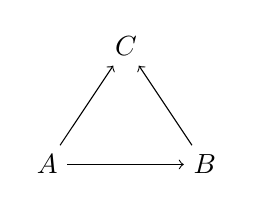
\begin{tikzpicture}
     % Nodes
     \node (A) at (0,0) {$A$};
     \node (B) at (2,0) {$B$};
     \node (C) at (1,1.5) {$C$};
     
     % Arrows
     \draw[->] (A) -- (B);
     \draw[->] (A) -- (C);
     \draw[->] (B) -- (C);
\end{tikzpicture}

% Commutative diagram
\begin{tikzpicture}
     \matrix (m) [matrix of math nodes,
     row sep=3em, column sep=4em]{
          X & Y \\
          Z & W \\
     };
     \path[->]
     (m-1-1) edge (m-1-2)
     edge (m-2-1)
     (m-1-2) edge (m-2-2)
     (m-2-1) edge (m-2-2);
\end{tikzpicture}
               \end{lstlisting}
          \end{column}
          
          \begin{column}{0.5\textwidth}
               \textbf{Basic diagram:}
               \begin{center}
                    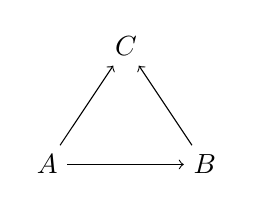
\begin{tikzpicture}
                         % Nodes
                         \node (A) at (0,0) {$A$};
                         \node (B) at (2,0) {$B$};
                         \node (C) at (1,1.5) {$C$};
                         
                         % Arrows
                         \draw[->] (A) -- (B);
                         \draw[->] (A) -- (C);
                         \draw[->] (B) -- (C);
                    \end{tikzpicture}
               \end{center}
               
               \textbf{Commutative diagram:}
               \begin{center}
                    \begin{tikzpicture}
                         \matrix (m) [matrix of math nodes,
                         row sep=3em, column sep=4em]{
                              X & Y \\
                              Z & W \\
                         };
                         \path[->]
                         (m-1-1) edge (m-1-2)
                         edge (m-2-1)
                         (m-1-2) edge (m-2-2)
                         (m-2-1) edge (m-2-2);
                    \end{tikzpicture}
               \end{center}
               
               \textbf{TikZ is powerful for:}
               \begin{itemize}
                    \item Commutative diagrams
                    \item Graphs and networks
                    \item Geometric figures
                    \item Custom illustrations
               \end{itemize}
          \end{column}
     \end{columns}
\end{frame}

\begin{frame}[fragile]{Custom Commands and Macros}
     \begin{columns}
          \begin{column}{0.5\textwidth}
               \begin{lstlisting}
% In preamble
% Simple command
\newcommand{\R}{\mathbb{R}}
\newcommand{\C}{\mathbb{C}}

% Command with parameter
\newcommand{\norm}[1]{\left\|#1\right\|}
\newcommand{\set}[1]{\{#1\}}

% Command with optional parameter
\newcommand{\derivative}[2][x]{
     \frac{d #2}{d #1}
}

% In document
Let $f: \R \to \R$ be a function.

The norm $\norm{v}$ of vector $v$.

The set $\set{1,2,3}$ contains 3 elements.

$\derivative{f}$ and $\derivative[t]{f}$
               \end{lstlisting}
          \end{column}
          
          \begin{column}{0.5\textwidth}
               \textbf{Benefits of custom commands:}
               \begin{itemize}
                    \item Consistent notation
                    \item Shorter source code
                    \item Easier to maintain
                    \item Can modify once, affects all instances
               \end{itemize}
               
               \textbf{Command types:}
               \begin{itemize}
                    \item \texttt{\textbackslash newcommand} - define new command
                    \item \texttt{\textbackslash renewcommand} - redefine existing
                    \item \texttt{\textbackslash providecommand} - only if not defined
               \end{itemize}
               
               \textbf{Parameters:}
               \begin{itemize}
                    \item Mandatory: \texttt{[1]} - number of parameters
                    \item Optional: \texttt{[1][default]} - with default
                    \item Access with \texttt{\#1}, \texttt{\#2}, etc.
               \end{itemize}
          \end{column}
     \end{columns}
     
     \begin{tip}
          Define math commands in the preamble for consistent notation throughout your document
     \end{tip}
\end{frame}

\begin{frame}[fragile]{Common Errors and Debugging}
     \begin{columns}
          \begin{column}{0.5\textwidth}
               \textbf{Common error messages:}
               
               \begin{lstlisting}[language={}]
                    ! Undefined control sequence.
                    l.10 \unkowncommand
                    
               \end{lstlisting}
               \textcolor{red}{Typo or missing package}
               
\begin{lstlisting}[language={}]
! Missing $ inserted.
l.15 The equation x^2
                    
\end{lstlisting}
               \textcolor{red}{Math command outside math mode}
               
               \begin{lstlisting}[language={}]
! LaTeX Error: Environment unknown 
undefined.
               \end{lstlisting}
               \textcolor{red}{Typo or missing package for environment}
               
               \begin{lstlisting}[language={}]
                    ! Missing \begin{document}.
                    \end{lstlisting}
                    \textcolor{red}{Text before \textbackslash begin\{document\}}
               \end{column}
               
               \begin{column}{0.5\textwidth}
                    \textbf{Other common errors:}
                    \begin{itemize}
                         \item Missing or extra braces \{\}
                         \item Unmatched environment \texttt{\textbackslash begin} / \texttt{\textbackslash end}
                         \item Missing or mismatched \$ in math mode
                         \item Undefined references or citations
                         \item Package conflicts
                    \end{itemize}
                    
                    \textbf{Debugging tips:}
                    \begin{itemize}
                         \item Look at line number in error message
                         \item Comment out sections to isolate problems
                         \item Add packages and commands incrementally
                         \item Use \texttt{\textbackslash usepackage\{syntonly\}} to check syntax without output
                         \item Use \texttt{\%} for comments to help debug
                    \end{itemize}
               \end{column}
          \end{columns}
          
          \begin{warning}
               Always read the first error first - fixing it might solve later errors
          \end{warning}
     \end{frame}
     
     \begin{frame}[fragile]{Tips for Mathematical Writing}
          \begin{columns}
               \begin{column}{0.5\textwidth}
                    \textbf{Spacing in math expressions:}
                    
                    \begin{lstlisting}
% Too cramped
$f(x)=x^2+2x+1$

% Better with spacing
$f(x) = x^2 + 2x + 1$

% Manual spacing when needed
\begin{align*}
  y &= x^2 \\
  &= (x+1)(x-1) + 1 \\
  &= x^2 - 1 + 1 \\
  &= x^2
\end{align*}

% Spacing commands
$a \, b \: c \; d \! e$
$p \quad q \qquad r$
                    \end{lstlisting}
               \end{column}
               
               \begin{column}{0.5\textwidth}
                    \textbf{Math spacing commands:}
                    \begin{itemize}
                         \item \texttt{\textbackslash,} - small space
                         \item \texttt{\textbackslash:} - medium space
                         \item \texttt{\textbackslash;} - large space
                         \item \texttt{\textbackslash!} - negative space
                         \item \texttt{\textbackslash quad} - 1em space
                         \item \texttt{\textbackslash qquad} - 2em space
                    \end{itemize}
                    
                    \textbf{Writing best practices:}
                    \begin{itemize}
                         \item Use punctuation in displayed equations
                         \item Include math notation in the flow of text
                         \item Be consistent with notation
                         \item Define symbols when first introduced
                         \item Use \texttt{\textbackslash text\{...\}} for text in math
                         \item Avoid \texttt{\$\$...\$\$} (use \texttt{\textbackslash[...\textbackslash]} instead)
                    \end{itemize}
               \end{column}
          \end{columns}
     \end{frame}
     
     \begin{frame}{Resources and Communities}
          \begin{columns}
               \begin{column}{0.5\textwidth}
                    \textbf{Documentation:}
                    \begin{itemize}
                         \item \textbf{Books:}
                         \begin{itemize}
                              \item "The \LaTeX\ Companion" (Mittelbach et al.)
                              \item "Mathematics into Type" (Swanson)
                              \item "\LaTeX\ for Complete Novices" (Talbot)
                         \end{itemize}
                         
                         \item \textbf{Online guides:}
                         \begin{itemize}
                              \item Overleaf Documentation
                              \item CTAN package documentation
                              \item LaTeX Wikibook
                              \item TeX Stack Exchange tutorials
                         \end{itemize}
                    \end{itemize}
               \end{column}
               
               \begin{column}{0.5\textwidth}
                    \textbf{Getting help:}
                    \begin{itemize}
                         \item TeX Stack Exchange
                         \item r/LaTeX subreddit
                         \item LaTeX Community forum
                         \item Overleaf learn resources
                    \end{itemize}
                    
                    \textbf{Useful tools:}
                    \begin{itemize}
                         \item Detexify - find symbols by drawing
                         \item LaTeX Table Generator
                         \item MathPix - convert images to LaTeX
                         \item LaTeX templates (journals, theses)
                    \end{itemize}
               \end{column}
          \end{columns}
          
          \begin{block}{Package documentation}
               Always check the documentation for packages you use:\\
               \texttt{texdoc packagename} (command line) or\\
               Visit \url{https://ctan.org/pkg/packagename}
          \end{block}
     \end{frame}
     
     \begin{frame}{Exercise 4: Final Document}
          \begin{practice}
               \textbf{Create a complete mathematical article that includes:}
               \begin{enumerate}
                    \item Title, author, abstract
                    \item Table of contents
                    \item Mathematical content with properly typeset equations
                    \item At least one theorem and its proof
                    \item A figure or diagram
                    \item A table
                    \item Cross-references to all elements
                    \item A bibliography with at least two references
               \end{enumerate}
          \end{practice}
          
          \textbf{Bonus goals:}
          \begin{itemize}
               \item Define a custom macro
               \item Include a TikZ diagram
               \item Format the document according to a journal style
          \end{itemize}
     \end{frame}
     
     \begin{frame}{Introduction to Beamer for Presentations}
          \begin{columns}
               \begin{column}{0.5\textwidth}
                    \textbf{Beamer basics:}
                    \begin{itemize}
                         \item LaTeX document class for presentations
                         \item Create professional slides with math
                         \item Similar syntax to regular LaTeX
                         \item Powerful theming and customization
                    \end{itemize}
                    
                    \textbf{Key Beamer environments:}
                    \begin{itemize}
                         \item \texttt{frame} - individual slide
                         \item \texttt{block}, \texttt{alertblock} - text boxes
                         \item \texttt{columns} - multicolumn layout
                         \item \texttt{itemize}, \texttt{enumerate} - lists
                    \end{itemize}
               \end{column}
               
               \begin{column}{0.5\textwidth}
                    \textbf{Themes and customization:}
                    \begin{itemize}
                         \item Presentation themes (Madrid, Berlin, etc.)
                         \item Color themes (dolphin, crane, etc.)
                         \item Font themes
                         \item Inner/outer themes
                    \end{itemize}
                    
                    \textbf{Special features:}
                    \begin{itemize}
                         \item Overlays and incremental builds
                         \item Transitions and animations
                         \item Notes for presenter
                         \item Handout mode
                    \end{itemize}
               \end{column}
          \end{columns}
          
          \begin{tip}
               This presentation was created with Beamer! You can look at the source code as a reference.
          \end{tip}
     \end{frame}
     
     \begin{frame}[fragile]{Basic Beamer Example}
          \begin{columns}
               \begin{column}{0.5\textwidth}
                    \begin{lstlisting}
 \documentclass{beamer}
 \usetheme{Madrid}
 \usecolortheme{dolphin}
 
 \title{My Presentation}
 \author{Your Name}
 \date{\today}
 
 \begin{document}
      
\\begin{frame}
\titlepage
\\end{frame}

\\begin{frame}{Outline}
\tableofcontents
\\end{frame}

\section{First Topic}

\begin{frame}{Mathematics}
   The equation:
   \begin{equation}
        E = mc^2
   \end{equation}
   
   \begin{itemize}
        \item<1-> First point
        \item<2-> Second point
        \item<3-> Third point
   \end{itemize}
\\end{frame}
   
\\end{document}
              \end{lstlisting}
         \end{column}
         
         \begin{column}{0.5\textwidth}
              \textbf{Key points:}
              \begin{itemize}
                   \item \texttt{\textbackslash documentclass\{beamer\}}
                   \item Slides are created with \texttt{frame} environment
                   \item Each frame needs a title with \texttt{\{title\}}
                   \item \texttt{<1->} notation for incremental display
                   \item All math commands work as usual
              \end{itemize}
              
              \textbf{Common elements:}
              \begin{itemize}
                   \item Title page with \texttt{\textbackslash titlepage}
                   \item Outline with \texttt{\textbackslash tableofcontents}
                   \item Sections and subsections
                   \item Math equations, tables, figures
              \end{itemize}
              
              
         \end{column}
    \end{columns}
\end{frame}
               